\documentclass[11pt]{article}

% --- arXiv-ready single-column article ---
\usepackage{iftex}
\ifpdftex
  \usepackage[utf8]{inputenc}
  \usepackage[T1]{fontenc}
  \usepackage{lmodern}
\else
  \usepackage{fontspec}
\fi
\usepackage[margin=1in]{geometry}
\usepackage{graphicx}
\graphicspath{{../figures/}}
\usepackage{booktabs}
\usepackage{amsmath,amssymb}
\usepackage{textcomp}
\usepackage{natbib}
\usepackage[hidelinks]{hyperref}
\usepackage{microtype}
\usepackage{caption}
\captionsetup{font=small,labelfont=bf}

% Unicode glyphs that appear in the prose -> portable macros (both engines)
\usepackage{newunicodechar}
\newunicodechar{Δ}{\ensuremath{\Delta}}
\newunicodechar{τ}{\ensuremath{\tau}}
\newunicodechar{μ}{\ensuremath{\mu}}
\newunicodechar{±}{\ensuremath{\pm}}
\newunicodechar{≈}{\ensuremath{\approx}}
\newunicodechar{≥}{\ensuremath{\geq}}
\newunicodechar{≤}{\ensuremath{\leq}}
\newunicodechar{→}{\ensuremath{\rightarrow}}
\newunicodechar{×}{\ensuremath{\times}}
\newunicodechar{·}{\ensuremath{\cdot}}
\newunicodechar{−}{\ensuremath{-}}
\newunicodechar{°}{\ensuremath{^\circ}}
\newunicodechar{Ż}{\.Z}

\title{\textbf{Where Liquid Networks Help, Hurt, and Fail to Train:\\ A Pre-Registered Boundary Map}}
\author{Olga \.Zydziak\\ \small Independent Research}
\date{2026-07-24}

\begin{document}
\maketitle

\begin{abstract}
\noindent Liquid neural networks --- continuous-time cores such as LTCs and their closed-form successor (CfC), wired with NCP/AutoNCP --- are claimed to grant perception-and-control policies greater robustness under distribution shift. We subject that claim to a pre-registered measurement program spanning three task regimes at core-parameter parity and equal training budget: open-loop classification (companion P0, PASTIS), open-loop onset detection (companion E6), and closed-loop control (state-loop, LiquidFlight v1.0; vision-loop, this work). In the richest regime --- a vision-in-the-loop fly-to-target twin with a perceptual-shift ladder --- no CfC arm reaches our pre-registered nominal-capability precondition (mean $\geq$90\% success at core parity of 27{,}648 $\pm$2\%) on either allowed learning rate, so the robustness claim is \emph{untestable under our precondition} and no gate arm was ever evaluated out of distribution (OOD) under the frozen criterion; the only OOD data is the pre-registered sanity calibration (Section~\ref{sec:instr}). Beneath that boundary we measure a \emph{trainability tax}: at identical budget, a GRU control reaches 100\% while the wired CfC peaks at 92\% (per-leg means up to 75.3\%, a 43\,pp seed spread) and the dense CfC caps at 65\%. We attribute trainability to wiring, localize a continuous-time $\Delta t$ implementation dependency, and contribute a reusable gate/precondition methodology with an arithmetic early-stopping rule. A negative result, pre-registered, maps where the mechanism can and cannot be measured.
\end{abstract}

\section{Introduction}
Continuous-time recurrent networks have become an attractive substrate for embodied perception and control. Liquid Time-Constant networks (LTCs) and their closed-form counterpart (CfC), especially when wired with Neural Circuit Policies (NCP/AutoNCP), have been reported to yield policies that generalize better under distribution shift than conventional gated recurrences such as GRUs. The most cited demonstration in the flight domain reports that a compact liquid policy attends to the task-relevant part of the visual scene and holds up under perceptual perturbation \citep{chahine2023flight}.

Two properties of that literature motivate this work. First, demonstrations are typically reported \textbf{without core-parameter parity} against a matched baseline and \textbf{without pre-registration} of the success criterion; a favorable curve is shown, but the counterfactual --- a same-budget, same-data baseline under a criterion fixed in advance --- is often absent. Second, the field does not report a \textbf{trainability layer}: whether the liquid core can be brought to competence at all, at parity, under a fixed budget, before any robustness question is even asked.

We take the claim seriously enough to try to falsify it under conditions it should survive. We build an honest twin --- identical encoder, identical head, identical data and budget, cores matched to within $\pm$2\% --- and we freeze the success criterion before measuring. This paper reports the vision-loop regime (phase~3) as the primary result and folds it into a portfolio-level \textbf{boundary map} with two companion regimes.

\paragraph{Contributions} (mapped to our claim register C1--C8):
\begin{itemize}
  \item A pre-registered vision-loop twin in which the robustness claim is \emph{untestable under our precondition} --- the deciding arm never qualifies, and we hold to zero OOD evaluations of any gate arm (C1).
  \item A measured \textbf{trainability tax} at parity: GRU 100\% vs.\ wired-CfC (peak 92\%, per-leg means up to 75.3\%) vs.\ dense-CfC (cap 65\%), at identical budget (C2).
  \item The finding that the boundary is \textbf{variance, not mean} --- seed instability is the object of measurement, echoing the companion P0 population spread (C3).
  \item A \textbf{wiring attribution}: AutoNCP makes the CfC trainable where the dense CfC caps (C4).
  \item Engineering findings on the continuous-time $\Delta t$ path and DAgger procedure (C5, C6).
  \item A transferable \textbf{methodology}: gates, preconditions, annexes with a stop rule, and arithmetic early resolution (C7); plus an instrument characterization (C8).
\end{itemize}

\section{Related Work}
\paragraph{Liquid networks.} Liquid Time-Constant networks model the hidden state as a continuous-time dynamical system whose time constants are themselves input-dependent, giving the network a natively continuous notion of elapsed time \citep{hasani2021ltc}. Their closed-form successor, the CfC, replaces the numerical ODE solve with a closed-form update that preserves the continuous-time gate while removing solver cost \citep{hasani2022cfc}. Neural Circuit Policies and their automatic wiring (AutoNCP) impose a sparse, structured connectivity on the recurrent core, inspired by biological circuits and reported to improve auditability and compactness \citep{lechner2020ncps}. The robustness claim we test derives largely from a flight-navigation demonstration in which a small wired liquid policy generalizes out of distribution and attends to task-relevant structure \citep{chahine2023flight}; we treat that claim as the hypothesis under test and its lineage as the object we reproduce at parity. Two of our arms --- a wired CfC (A\_NCP) and a dense CfC (A\_CFC) --- are chosen precisely to isolate the contribution of the wiring from that of the continuous dynamics.

\paragraph{Continuous-time and state-space cousins.} Deep state-space models share the continuous-time framing: S4 parameterizes long-range dependencies through a structured state-space kernel \citep{gu2022s4}, Mamba adds input-dependent selectivity for linear-time sequence modeling \citep{gu2023mamba}, and Liquid-S4 connects the liquid formulation to this family \citep{hasani2023liquids4}. These situate our small recurrences within a broader continuous-time lineage; we do not evaluate them here.

\paragraph{Pre-registration, reproducibility, and imitation learning.} Our methodology adopts the discipline of freezing success criteria before measurement and reporting honest baselines, in the spirit of the machine-learning reproducibility and pre-registration literature \citep{pineau2021reproducibility,sogaard2023preregistration}. Training uses behavioral cloning followed by DAgger, the canonical no-regret reduction of imitation learning to online learning \citep{ross2011dagger}; a central engineering finding of this work concerns the interaction between the DAgger update mode and continuous-time cores (Section~\ref{sec:eng}). The vision harness is built on gym-pybullet-drones \citep{panerati2021gym}, and the companion open-loop regime uses the PASTIS satellite time-series benchmark \citep{garnot2021pastis}.

\section{The Measurement Program}\label{sec:program}
The program is a house methodology applied uniformly across regimes.

\paragraph{Honest twin.} Each arm shares the same encoder, the same \texttt{Linear(64$\to$6)} head with identical output scaling, the same training data and budget; cores are matched to a reference of 27{,}648 core parameters to within $\pm$2\%. The only sanctioned inter-arm difference is the learning rate, whose provenance is documented.

\paragraph{Frozen criteria; MEASURE = REPORT.} Success criteria are frozen in a gate document before any measurement; whatever is measured is reported, including nulls and boundaries. The vision-loop gate (F3-GATE) fixes the OOD level (T2b), the primary metric, the decision threshold, and $n$ before any thesis measurement.

\paragraph{Gates and preconditions.} A capability \textbf{precondition} (nominal success $\geq$90\% per arm) must pass before the thesis metric is evaluated; the precondition is \emph{not} the thesis. Failing it triggers a sanctioned, nominal-only repair (a learning rate from the pre-registered fallback grid --- nothing else) and a full retrain, logged; exhaustion is a STOP for a human decision, not a verdict on the thesis.

\paragraph{Annexes with a stop rule.} When the recipe diverges from a frozen, known-good reference, we unfreeze via an \textbf{annex} that cites the reference line-by-line and applies the change symmetrically to all arms. The stop rule (Annex-4) declares the last instrumental annex of phase~3a: if a CfC arm still fails the precondition afterward, FAIL becomes a reported \textbf{boundary}, not another annex.

\paragraph{Arithmetic early resolution.} Because the precondition is a mean over 10 seeds, a leg can be resolved before all seeds run: after $k$ seeds summing to $S$, if $S + (10-k)\cdot 100 < 900$ the leg cannot reach 90\% and is declared FAIL. This is arithmetic on the frozen criterion, not a change to it. In phase~3 it reduced the run to \textbf{13 full cycles instead of 40} and left one four-seed batch never launched (Appendix~\ref{app:early}).

\paragraph{Determinism contract.} Environment, rendering, and seeding are bit-exact reproducible \textbf{within a single machine} (two runs, rgb/kin/setpoint identical). Cross-machine hashes may differ and that is not a failure --- determinism is a within-machine property, not a cross-machine guarantee.

\section{Harnesses}
The portfolio uses three instruments, one per regime.

\paragraph{4.1 PASTIS twin (P0).} Sentinel-2 crop classification of a phenologically confusable pair (soft winter wheat vs.\ corn) under test-time observation dropout, with a shared CNN encoder (28{,}752 parameters) and only the recurrent core swapped between CfC and GRU. Open-loop, day-scale. Companion; numbers verified against the companion report \citep{zydziak2026p0}.

\paragraph{4.2 LiquidFlight (state-loop, v1.0).} A closed-loop drone flight twin (gym-pybullet-drones \citep{panerati2021gym}) with a setpoint$\to$DSL-PID inner loop at 48\,Hz, an observation-dropout OOD axis and a gap-length (latency) axis, and a time-constant ($\tau$) inspection panel; CfC(32) vs.\ GRU at core parity, everything but the core bit-identical between arms. The vision-loop harness reuses this execution layer verbatim (sha256-pinned copies).

\paragraph{4.3 LiquidSight (vision-loop, phase 3 --- this work).} A fly-to-target task from a $64\times64\times3$ forward camera plus kinematics: reach a ground marker and hold a hover within \texttt{r\_goal} for the final dwell window. Physics at 240\,Hz, control at 48\,Hz, camera and policy tick at 12\,Hz; the target lives only in pixels. A privileged DSL-PID expert supplies behavioral cloning (BC) labels; three DAgger rounds follow. The perceptual-shift axis is a distractor ladder T0--T3 (T2/T2a/T2b/T2c $= K\in\{0,1,2,3\}$ distractors on structured backgrounds), with P-SANITY establishing that the axis resolves difficulty and that the expert ceiling is reachable at every level (Section~\ref{sec:instr}). The gate level is T2b.

\section{Results Across Regimes}\label{sec:results}
The boundary map (Table~\ref{tab:map}) summarizes the direction and measurement resolution of the effect in each regime. No measurement crosses its pre-registered threshold.

\begin{table}[h]
\centering
\small
\caption{Boundary map across task regimes.}\label{tab:map}
\begin{tabular}{llll}
\toprule
row & regime / harness & effect direction & verdict / resolution \\
\midrule
R1 & open-loop classification (P0) & weak positive under dropout & null (margin $<$ pooled std); quantitative \\
R2 & onset detection, low FAR (E6) & \textbf{negative} & directional; qualitative (secondary source) \\
R3 & state-loop control (v1.0) & zero & quantitative \\
R4 & vision-loop (this work) & untestable under precondition & precondition FAIL at parity; quantitative \\
\bottomrule
\end{tabular}
\end{table}

\subsection{Vision-loop (phase 3) --- the primary result}
\paragraph{The robustness claim is untestable under our precondition (C1).} After restoring the known-good recipe in full (core construction, Annex-3; training procedure, Annex-4) and exhausting the only sanctioned lever --- the learning-rate grid $\{$3e-4, 1e-3$\}$ --- \textbf{no CfC arm reaches the pre-registered precondition} of mean $\geq$90\% nominal success at core parity. All four lr legs resolve to FAIL by arithmetic early resolution: A\_NCP at 3e-4 $=$ 16.5\% (resolved at $k{=}2$), A\_NCP at 1e-3 $=$ \textbf{72.2\%} ($k{=}4$), A\_CFC at 3e-4 $=$ 27.0\% ($k{=}2$), A\_CFC at 1e-3 $=$ 55.3\% ($k{=}3$). Because the \textbf{deciding arm} (A\_NCP, the AutoNCP-wired CfC faithful to the wiring in the cited claim) does not qualify, the thesis metric --- a T2b margin of A\_NCP over A\_GRU with threshold $M > \text{pooled\_std}$, $n{=}10$ --- is \emph{untestable under our precondition}. We therefore ran \textbf{zero OOD evaluations of any gate arm} in the entire phase: gate stages B (the A\_GRU precondition sweep) and C (the OOD ladder) were skipped by the branch, so the pre-registered verdict remains untouched and unprejudiced. The only out-of-distribution data seen anywhere in the phase is the pre-registered sanity calibration of the perceptual-shift axis (the P-SANITY ladder), which is a pre-gate instrument check, not a thesis measurement (Section~\ref{sec:instr}).

This is deliberately \emph{not} a falsification of the thesis. A test requires a qualifying deciding arm; without the precondition there is no test. The result is a cell in the boundary map, not a verdict on the mechanism.

\begin{figure}[h]
\centering
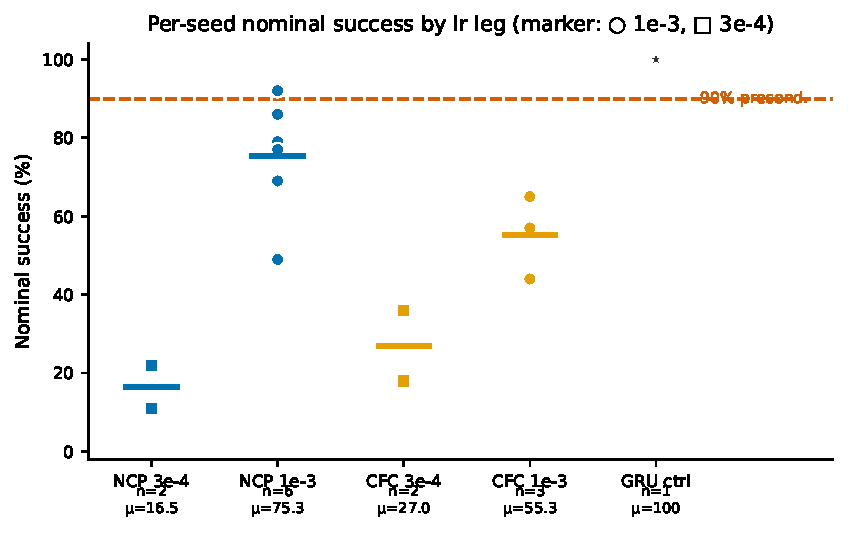
\includegraphics[width=0.8\linewidth]{fig_b_perseed_nominal.pdf}
\caption{\emph{Per-seed nominal success for each lr leg.} Points show nominal success (100 scenes, level T0) for every trained seed across the four CfC lr legs (A\_NCP and A\_CFC $\times$ $\{$3e-4, 1e-3$\}$); horizontal bars mark per-leg means; a dashed rule marks the 90\% precondition. The A\_GRU control (100\%) is shown for reference. The wired arm at 1e-3 spans 49--92\% (43\,pp); no leg mean crosses 90\%.}
\end{figure}

\paragraph{A trainability tax at parity (C2).} At identical data, budget, and procedure, and with cores matched to $\pm$2\%, nominal capability forms a gradient: \textbf{A\_GRU 100\%} (stable; dwell failures 0; 100\% in every GRU training of the program: P-SANITY, the procedure-v1 smoke, and the procedure-v2 smoke ($=$ the binding control)) $>$ \textbf{wired CfC} (A\_NCP; peak 92\% at seed 45010/1e-3; per-leg mean 72.2\% at $k{=}4$) $>$ \textbf{dense CfC} (A\_CFC; cap 65\% at seed 45012/1e-3). Core-parameter parity alone does not buy capability; the continuous-time core pays a trainability tax at this budget. The dominant residual failure is \textbf{dwell} --- the drone reaches the marker but does not hold the hover precisely --- while catastrophic \textbf{tilt is eliminated} at 1e-3 (0 tilt across all CfC cycles, versus 78/100 for the dense CfC under the pre-Annex-4 procedure).

\paragraph{The boundary is variance, not mean (C3).} The wired arm at 1e-3 spans \textbf{49--92\% across seeds --- a 43\,pp spread} --- under one fixed procedure, while the GRU control is a stable 100\%. Reporting only the $k{=}4$ mean (72.2\%) understates the phenomenon; the \textbf{full six-seed characterization (75.3\%, spread 43\,pp)} shows the boundary is a property of the between-seed distribution, not a sample-size artifact. The CfC at parity does not ``fail to learn''; it learns \textbf{unstably and dwell-limited, on average below 90\%}. This mirrors the companion P0 result \citep{zydziak2026p0}, where the retention margin ($+0.1127$) and its pooled standard deviation ($0.1759$) are nearly invariant between $n{=}3$ and $n{=}15$ --- population spread that does not shrink with $n$.

\paragraph{Wiring attribution (C4).} The contrast between arms attributes trainability to the wiring: the AutoNCP-wired CfC reaches a 92\% peak and per-leg means up to 75.3\%, whereas the dense CfC caps at 65\%, across seeds and at the 1e-3 lever. The attribution holds on the 1e-3 lever; at 3e-4 the ordering inverts (dense 27.0\% $>$ wired 16.5\%), so the wiring benefit is itself learning-rate dependent and we report it as such. A historical, single-seed diagnostic corroborates the readout dimension: reading the full state rather than six motor neurons raises reach from 8/50 to 26/50 (Section~\ref{sec:eng}).

\begin{figure}[h]
\centering
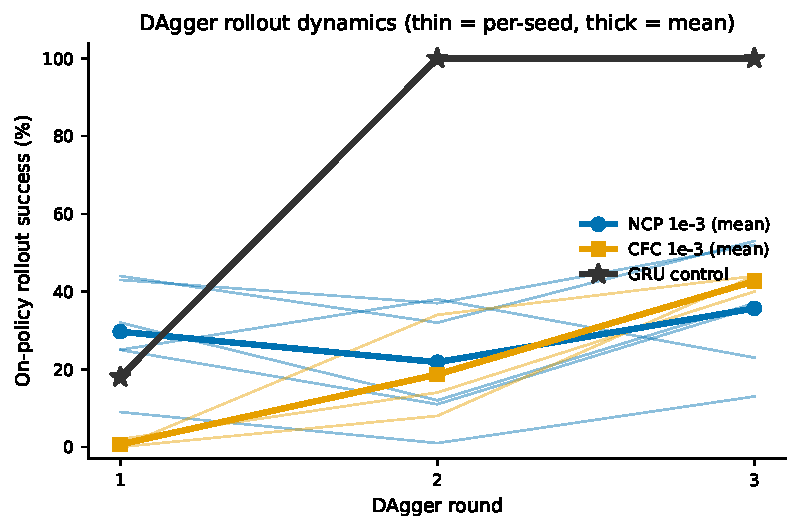
\includegraphics[width=0.75\linewidth]{fig_c_dagger_rollout.pdf}
\caption{\emph{DAgger rollout dynamics per round.} On-policy rollout success across DAgger rounds r1$\to$r2$\to$r3. The GRU control climbs 18$\to$100$\to$100; CfC arms stay low or flat, illustrating that the aggregate does not close for the continuous-time cores (thin: per-seed; thick: per-leg mean).}
\end{figure}

\subsection{Open-loop classification, day-scale (P0) --- companion}
The PASTIS twin gives a directional-but-null signal: at full cadence the GRU leads on macro-F1 (0.9073 $\pm$0.0137 vs.\ 0.8802 $\pm$0.0121), but under observation dropout the CfC retains more --- retention $R(0.6)$ of 0.6415 $\pm$0.1138 vs.\ 0.5288 $\pm$0.0622, a \textbf{$+0.1127$ margin against a pooled std of 0.1759, i.e.\ null} by the pre-registered rule. An absolute-F1 crossover appears at $d{=}0.6$ (CfC 0.5642 $\pm$0.0985 above GRU 0.4798 $\pm$0.0567, despite a $-0.027$ start), and the degradation slope is gentler for the CfC ($-0.5095$ vs.\ $-0.6936$). Crucially, margin and pooled std are near-invariant from $n{=}3$ to $n{=}15$ --- the boundary is population spread, not sampling noise. All P0 numbers are verified against the companion report \citep{zydziak2026p0}.

\subsection{Open-loop onset detection, low FAR (E6) --- companion}
The onset-detection regime contributes the \textbf{negative direction} of the map: at a low false-alarm-rate operating point the effect sign is \textbf{unfavorable to the liquid core}, as recorded in the program compendium; the primary E6 report is not preserved in the project archive. We therefore state this regime \textbf{qualitatively only} and report no numerical values for it --- in particular the detection-delay delta, the sweep parameter, and the false-alarm-rate definition are not carried into the prose, since their primary source could not be verified. The regime enters the boundary map as a directional cell (Table~\ref{tab:map}, row R2), not as a quantitative result.

\subsection{State-loop control, millisecond-scale (LiquidFlight v1.0) --- companion}
In the state-loop regime the continuous-time lever ($\Delta t$) is not behaviorally load-bearing. With a setpoint action abstraction the CfC-32 policy flies under 500--1300\,ms observation gaps and the episode-failure cliff moves from $\approx$102\,ms (raw-RPM stabilization) to $\approx$779\,ms; the $\Delta t$ mechanism is \emph{visible} in the state dynamics (recovery after a gap) but yields \textbf{no behavioral edge} --- ablating the $\Delta t$ channel flies identically. The fitted time constants are short (median $\tau \approx 35$\,ms, IQR 24--69\,ms), so a 500\,ms gap is $\approx$14$\times$ $\tau$ and the model does not bridge gaps with long memory; $\tau$ serves as an explainability handle, not a source of advantage. Under the A1 perturbation grid there were \textbf{0 tip-overs}. The regime contributes a \textbf{zero} to the map: neither help nor harm attributable to the liquid core at this horizon.

\section{Engineering Findings}\label{sec:eng}
Bringing a CfC to the point where it will run at all in this harness required restoring a known-good recipe in four provenanced steps (fixes \textbf{F1--F4}); each is an \textbf{engineering finding, established by single-seed controlled probes (diagnostic, not statistical)} --- not a statistically powered ablation.

\paragraph{F1 --- Backbone.} The dense CfC built without a backbone under the parity constraint does not reach the target (reach 8/50); adding a frozen-style backbone restores it (35/50, $\approx$ GRU) (Annex-3).

\paragraph{F2 --- The $\Delta t$ path and its units (C5).} The continuous-time core --- the sole locus of the thesis mechanism --- is load-bearing only after two corrections. First, the time-span scale sets the gate regime: with an explicit \texttt{ts} in \textbf{seconds} (0.0833\,s per 12\,Hz tick) reach is 39/50, versus 15/50 at ts$=$1.0 (ticks) and 9/50 at ts$=$4.0; the post-init gate drive $|t_a\cdot\text{ts}|$ scales accordingly (0.010 / 0.125 / 0.501), so a mis-scaled \texttt{ts} freezes or destabilizes the cell. Second, we found a \textbf{library bug}: \texttt{ncps.torch.CfC} rejects explicit \texttt{timespans} when the batch size exceeds one (scalar, $(B,1)$, and $(B,)$ all raise; only \texttt{None}$=$1.0 works), which had trapped the arms at ts$=$1.0. We work around it by stepping the cell manually. The auxiliary thesis is therefore: \textbf{$\Delta t$ is load-bearing implementationally, not advantageously} --- in this harness we could not measure an advantage because the precondition was never met.

\paragraph{F3 --- Full-state readout.} Reading the wired core's full state rather than six motor neurons lowers BC error (0.0047 vs.\ 0.0220) and raises reach (26/50 vs.\ 8/50) (Annex-3).

\paragraph{F4 --- DAgger update mode (C6).} Continuous-time cells are sensitive to the DAgger update procedure. Under the gate's original v1 mode (continue from the previous weights $+$ final-epoch checkpoint), the dense CfC becomes unstable (tilt 78/100) and the wired CfC collapses its rollouts (1$\to$0$\to$0); the dense CfC is stable after BC alone (0 tilt), so the instability is \textbf{induced by the procedure}, not the construction. Adopting the frozen-C1 mode symmetrically (retrain from scratch each round $+$ best-validation checkpoint, 120 epochs per stage; Annex-4) removes the tilt (78$\to$0 at 1e-3) and follows the canonical DAgger formulation \citep{ross2011dagger}. The \textbf{GRU is robust to both procedures} (100\% either way).

A mechanistic signature accompanies this (C6a): for every CfC arm the best validation error after BC alone is low ($\approx$0.00012--0.0009) but \textbf{rises} after the DAgger aggregate (rounds r1--r3), and the best epoch moves early (e.g., wired at 1e-3, seed 45013: 119$\to$41$\to$26$\to$37) --- the core does not close the fit to the policy-visited distribution as well as it fits the clean expert. The GRU holds its best validation low across all rounds (.000168$\to$.000112) --- a different regime.

\begin{figure}[h]
\centering
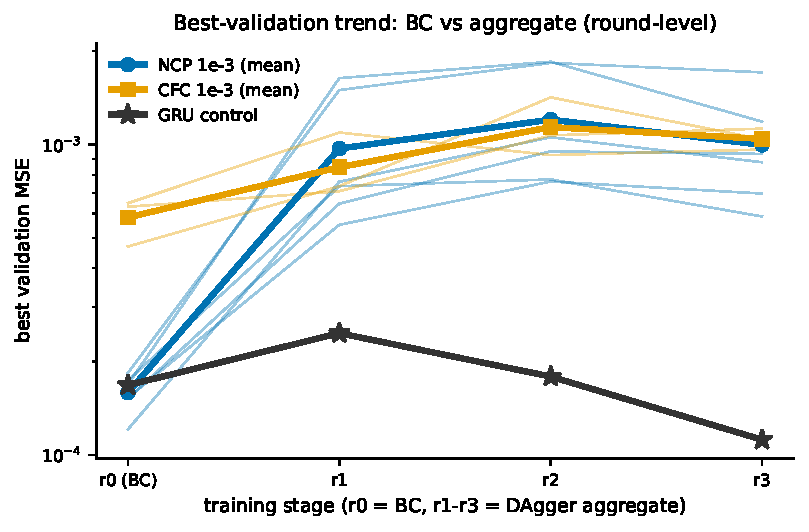
\includegraphics[width=0.75\linewidth]{fig_e_bestval_trend.pdf}
\caption{\emph{Best-validation trend, BC vs.\ aggregate.} Best validation MSE per stage (r0 $=$ BC $\to$ r1--r3 $=$ DAgger aggregate) for the CfC arms (rising after aggregation, best epoch moving earlier) against the GRU control (monotonically low). Round-level (four points per cycle); full per-epoch curves are not persisted and would require re-measurement.}
\end{figure}

\section{Instrument Characterization and Protocol Economics}\label{sec:instr}
\paragraph{Axis resolution and expert ceiling (C8).} The perceptual-shift axis resolves difficulty monotonically. The sanity policy degrades \textbf{100/100/64/46/36/24/16} across T0/T1/T2/T2a/T2b/T2c/T3 (50 scenes per level), placing three levels inside the pre-registered [30\%, 85\%] band and selecting \textbf{T2b (36\%)} as the hardest in-band gate level. The privileged expert reaches a \textbf{100\% ceiling at every level}, confirming that the distractors do not block physical reachability --- the axis touches pixels only. Determinism is bit-exact \textbf{within a machine} (rgb/kin/setpoint identical across two runs; cross-machine equality is neither required nor claimed).

\begin{figure}[h]
\centering
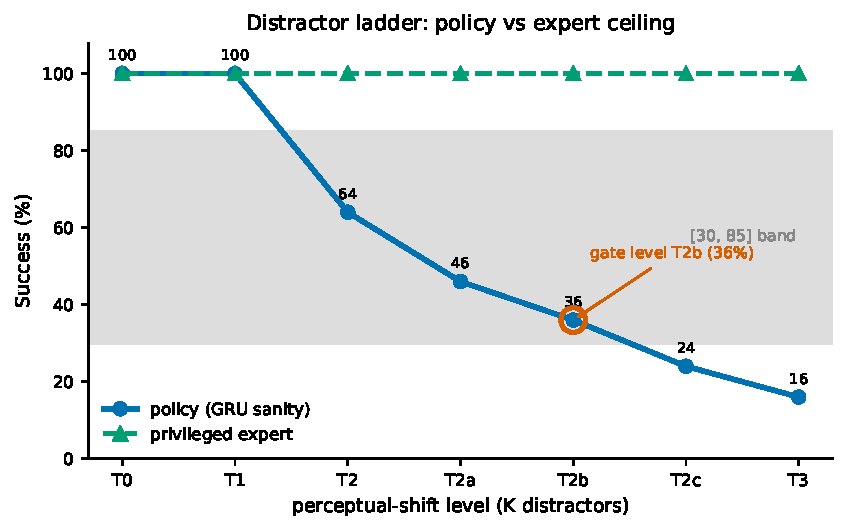
\includegraphics[width=0.75\linewidth]{fig_d_ladder_expert.pdf}
\caption{\emph{Sanity ladder and expert ceiling.} Policy success across the distractor ladder (T0$\to$T3: 100/100/64/46/36/24/16) with the [30,85] band shaded and the T2b gate level marked; the expert ceiling (100\% at every level) overlaid.}
\end{figure}

\paragraph{Protocol economics (C7a).} The binding run comprised \textbf{13 full training cycles} (plus one GRU control), $\approx$\textbf{57.1\,h} of cumulative compute. Per-cycle wall times in the binding run are inflated by GPU contention (3--6 concurrent processes on one GPU). Solo-cycle costs were measured only for the GRU control and the 3e-4 legs (\textbf{1.7--2.4\,h per cycle}); the 1e-3 CfC legs ran only under contention, so their solo cost is unmeasured. The 57.1\,h figure is therefore a \emph{sum of contention-inflated per-cycle times}, not a serial wall-clock (Table~T7). Arithmetic early resolution spared a complete four-seed batch relative to the 40 cycles a full $n{=}10$ over four legs would have required.

\section{Discussion}
\paragraph{Synthesis.} Across the regimes we map, the sign of the effect depends on the task: a weak positive in sparse open-loop observation (P0), a negative under low-FAR onset detection (E6), a zero in state-loop control (LiquidFlight), and --- in the richest regime, vision-in-the-loop --- a question that never reaches the conditions of measurement, because the advantage is preceded by a trainability tax at parity. No measurement crosses its pre-registered threshold. The unifying reading is that \textbf{task construction decides whether the mechanism can reveal itself at all}: the continuous-time core needs a regime whose dependencies it is positioned to exploit, and at parity it must first be trainable there.

\paragraph{Demonstration culture vs.\ falsification.} A pre-registered null carries evidential weight that a single favorable curve does not. Much of the liquid-network robustness literature is demonstrated rather than falsified: a favorable model is shown on a task chosen after the fact, without a same-budget parity baseline and without a criterion fixed in advance. Our program inverts that stance --- it commits to a threshold, a level, and a seed count before any out-of-distribution scene is seen, and it reports whatever the instrument returns, including a boundary. The cost of this discipline is that we sometimes conclude ``untestable'' rather than ``wins'' or ``loses''; the benefit is that the three cells we \emph{can} state (weak-positive, negative, zero) are not artifacts of selective reporting. The map says where to look and where not to --- it does not claim the mechanism is absent, only that under parity, fixed budget, and frozen criteria we did not measure it in these harnesses.

\paragraph{When the twin re-arms.} The vision-loop cell would re-enter measurement under conditions that unlock trainability without breaking parity. The cleanest such condition is a \textbf{symmetric budget increase} for all arms --- more epochs, more DAgger rounds, or more data applied identically to GRU and CfC --- carried until the deciding arm (A\_NCP) meets the precondition; the wired arm at 1e-3 is the natural starting point, already at 92\% best seed and 75.3\% mean. Because the increase is symmetric, the duel remains fair: if the GRU also improves, the parity contract is preserved. Two subsidiary questions gate the value of that rerun. First, the sensitivity of continuous-time cells to the DAgger update mode (F4) is an open research problem worth isolating on its own --- why does retrain-from-scratch with best-validation selection stabilize a CfC that continuation destabilizes, when a GRU is indifferent to both? Second, whether the residual dwell failure reflects a precision limit of the continuous-time state under this readout, or merely under-training, is answerable only once the precondition is met. Until then, we resist reading the boundary as evidence about the mechanism itself.

\paragraph{Next habitat.} The mechanism's most plausible next habitat is a regime with genuinely variable time steps or asynchronous/event-stream sensing, where the continuous-time gate has something to integrate --- offered as a direction, not a promise.

\section{Limitations}
\begin{itemize}
  \item \textbf{Simulation only.} PyBullet dynamics, no photorealism, no sim-to-real transfer.
  \item \textbf{One harness per regime.} A single fly-to-target task family at $64\times64$; results may not generalize across task families.
  \item \textbf{Parity at $\approx$27k core parameters.} Findings are stated at this capacity; other capacities are untested.
  \item \textbf{$n{=}10$ with a finality rule.} Seeds 45010--45015 were used (early resolution); increasing $n$, or changing the level or threshold after seeing any OOD result, is forbidden by the gate.
  \item \textbf{No OOD measurement of any gate arm in the vision-loop regime.} This is a \emph{consequence} of the unmet precondition, not a design choice; the only OOD data anywhere in the phase is the pre-gate sanity calibration.
  \item \textbf{Single-cycle GRU control.} The binding-run GRU control is a single cycle, corroborated by two earlier independent 100\% cycles.
  \item \textbf{Engineering findings are single-seed probes.} The four recipe restorations (fixes F1--F4) are diagnostic controlled probes ($n{=}1$ for most), illustrative rather than statistically powered.
  \item \textbf{Determinism is within-machine}, not cross-machine.
  \item \textbf{Fixed training budget.} The trainability tax is measured at BC-120 $+$ DAgger$\times$3; a higher symmetric budget is unmeasured.
  \item \textbf{Single-operator program}; one task family per regime.
  \item \textbf{Companion E6 primary report not preserved.} The onset-detection regime (R2) is stated qualitatively from a secondary source; its primary report is absent from the archive, so R2 carries no numerical values and its direction should be read as directional evidence, not a measured effect size.
\end{itemize}

\section{Reproducibility and Artifacts}
The liquidflight v1.0 and liquidsight repositories (tags and gate commits), the frozen documents (F3\_PRE0, decisions and Annexes 1--4, P-SANITY, F3-GATE), sha256 manifests of the execution layer, the seed pools, the per-cycle logs, and the reports \textbf{will be released upon publication}. The companion P0 ships as a separate PDF/arXiv artifact \citep{zydziak2026p0}. Instrument determinism is within-machine bit-exact; bit-for-bit reproduction across different GPUs is not guaranteed (inherent to CUDA).

\section{Conclusion}
We set out to test a robustness claim about liquid networks and, in the richest regime, found the claim \textbf{untestable under our pre-registered precondition}: at core parity and fixed budget, no continuous-time arm becomes reliably competent, so no out-of-distribution verdict can be earned. The first-order result is therefore a \textbf{boundary map} --- where the mechanism helps (weakly), hurts, is neutral, and cannot yet be measured --- together with a \textbf{trainability tax} that the field does not usually report: a same-budget capability gradient from a stable GRU (100\%) through a wired CfC (peak 92\%) to a dense CfC (cap 65\%). The measurement methodology --- gates, preconditions, provenanced annexes with a stop rule, and arithmetic early resolution --- is the portable contribution. A negative result, pre-registered, is a map of where to measure next.

\appendix
\section{Program timeline}\label{app:timeline}
\begin{figure}[h]
\centering
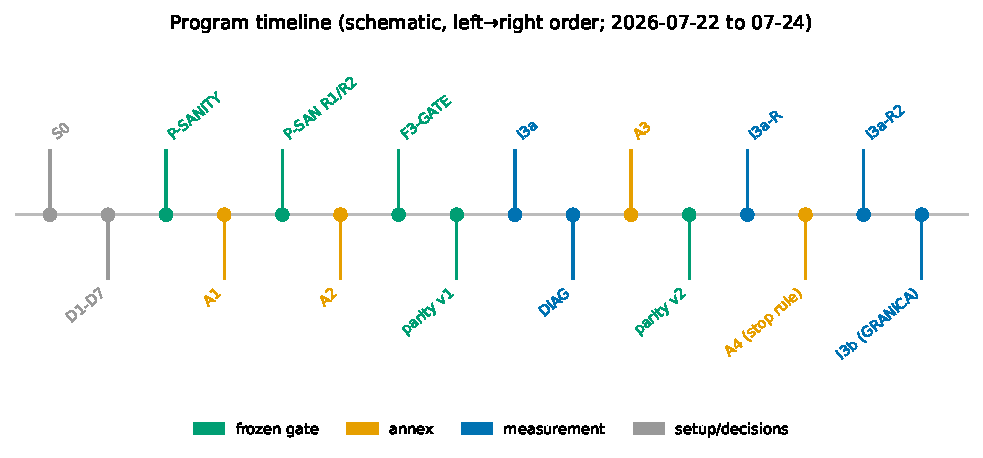
\includegraphics[width=\linewidth]{fig_a_timeline.pdf}
\caption{\emph{Gate and annex timeline.} The phase-3 program as a left-to-right order (2026-07-22 to 07-24): frozen gates (P-SANITY, F3-GATE, parity v1/v2), annexes (A1 observability, A2 distractor ladder, A3 core construction, A4 training procedure), and measurements (I3a, DIAG, I3a-R, I3a-R2, I3b).}
\end{figure}
One-line reasons: \textbf{Annex-1} spawned the target in the frontal cone and pitched the camera $-22.3^\circ$ so the marker is in-frame; \textbf{Annex-2} extended the axis with T2a/T2b/T2c (K$=$1/2/3) to fill resolution; \textbf{Annex-3} fixed three CfC construction defects (backbone, ts-in-seconds, full-state readout); \textbf{Annex-4} unified the training procedure with frozen C1 (from-scratch per round, best-val, 120 epochs) and declared the stop rule.

\section{Frozen criteria (pointers)}
\begin{itemize}
  \item \textbf{P-SANITY}: P1 capability $\geq$90\%; P2 axis resolution $\geq$2 levels in [30,85]; P3 expert ceiling $\geq$95\%/level.
  \item \textbf{F3-GATE \S4}: precondition mean nominal success $\geq$90\% per arm; fallback grid $\{$3e-4, 1e-3$\}$; no OOD before all arms pass.
  \item \textbf{F3-GATE \S5}: primary metric $M = \text{mean}_s\,\text{succ}(\text{A\_NCP},s) - \text{mean}_s\,\text{succ}(\text{A\_GRU},s)$, $n{=}10$; $\text{pooled\_std} = \sqrt{(\text{sd}(\text{A\_NCP})^2 + \text{sd}(\text{A\_GRU})^2)/2}$; verdict $M > \text{pooled\_std}$; binding at $n{=}10$.
  \item \textbf{Stop rule} (Annex-4): the last instrumental annex of phase 3a; a subsequent precondition FAIL becomes a reported boundary.
\end{itemize}

\section{Per-seed tables (binding run I3b)}\label{app:perseed}
Columns: nominal \% $\mid$ failures $\mid$ DAgger rollout r1$\to$r2$\to$r3 $\mid$ best-val r0$\to$r3 $\mid$ best-epoch $\mid$ cycle seconds. Generated from the per-cycle log (read, not measured).

\begin{table}[h]
\centering\small
\caption{A\_NCP @ 1e-3 (best leg; mean 72.2\% at $k{=}4$, 75.3\% over six seeds, 43\,pp spread).}
\begin{tabular}{rrlllr}
\toprule
seed & nom\% & failures & rollout & best-val r0$\to$r3 & sec \\
\midrule
45010 & 92 & dwell 8 & 44$\to$32$\to$53 & .000174$\to$.000587 & 18{,}889.3 \\
45011 & 79 & dwell 21 & 43$\to$37$\to$52 & .000153$\to$.000696 & 19{,}138.1 \\
45012 & 69 & dwell 31 & 25$\to$11$\to$36 & .000169$\to$.001187 & 19{,}441.2 \\
45013 & 49 & dwell 51 & 9$\to$1$\to$13 & .000184$\to$.001711 & 18{,}986.6 \\
45014 & 86 & dwell 14 & 32$\to$12$\to$37 & .000121$\to$.000878 & 19{,}471.4 \\
45015 & 77 & dwell 23 & 25$\to$38$\to$23 & .000152$\to$.000934 & 18{,}992.2 \\
\bottomrule
\end{tabular}
\end{table}

\begin{table}[h]
\centering\small
\caption{Other legs and the GRU control (procedure v2).}
\begin{tabular}{llrrll}
\toprule
leg & seed & nom\% & failures & rollout & best-val r0$\to$r3 \\
\midrule
A\_NCP 3e-4 & 45010 & 22 & dwell 76, tilt 2 & 22$\to$13$\to$25 & .000566$\to$.001843 \\
A\_NCP 3e-4 & 45011 & 11 & dwell 89 & 12$\to$0$\to$12 & .000721$\to$.002428 \\
A\_CFC 1e-3 & 45010 & 44 & dwell 56 & 0$\to$8$\to$44 & .000648$\to$.000965 \\
A\_CFC 1e-3 & 45011 & 57 & dwell 43 & 2$\to$14$\to$40 & .000631$\to$.001127 \\
A\_CFC 1e-3 & 45012 & 65 & dwell 35 & 0$\to$34$\to$44 & .00047$\to$.001041 \\
A\_CFC 3e-4 & 45010 & 18 & dwell 70, tilt 12 & 8$\to$0$\to$6 & .000887$\to$.002938 \\
A\_CFC 3e-4 & 45011 & 36 & dwell 64 & 2$\to$0$\to$8 & .000889$\to$.002709 \\
A\_GRU 1e-3 & 45010 & 100 & --- (dwell 0) & 18$\to$100$\to$100 & .000168$\to$.000112 \\
\bottomrule
\end{tabular}
\end{table}

\section{Early-resolution formula and savings}\label{app:early}
For a per-arm precondition of mean $\geq$90\% over 10 seeds, after $k$ seeds with partial sum $S$ the leg is declared FAIL when
\[ S + (10-k)\cdot 100 < 900. \]
Applied to the four legs: A\_NCP@3e-4 FAIL at $k{=}2$ ($S{=}33$; $833<900$); A\_NCP@1e-3 FAIL at $k{=}4$ ($S{=}289$; $889<900$); A\_CFC@3e-4 FAIL at $k{=}2$ ($S{=}54$; $854<900$); A\_CFC@1e-3 FAIL at $k{=}3$ ($S{=}166$; $866<900$). Total executed: 13 cycles versus 40 for a full $n{=}10$ over four legs; one four-seed batch (45016--45019) was never launched. This is arithmetic on the frozen criterion, not a modification of it.

\bibliographystyle{plainnat}
\bibliography{references}

\end{document}
